\section {Функция <<Лисьи норы>> Шекеля}
\label{TestFunctions:section:HML_TestFunction_ShekelsFoxholes}
\subsection {Описание функции}

\begin{tabularwide}
\textbf{Идентификатор:} & HML\_TestFunction\_ShekelsFoxholes. \\
\textbf{Наименование:} & Функция <<Лисьи норы>> Шекеля. \\
\textbf{Тип:} & Задача вещественной оптимизации. \\
\end{tabularwide}

\textbf{Формула} (целевая функция):
\begin{equation}
\label{TestFunctions:eq:HML_TestFunction_ShekelsFoxholes}
f\left( \bar{x}\right) = \dfrac{1}{\dfrac{1}{K}+\sum_{j=1}^{25}\dfrac{1}{j+\left( \bar{x}_1-A_{1,j}\right)^6+ \left( \bar{x}_2-A_{2,j}\right)^6}}, \text{ где}
\end{equation}
\indent $\bar{x}\in X$, $\bar{x}_j\in \left[ Left_j; Right_j\right] $, $Left_j=-50$, $Right_j=50$, $j=\overline{1,n}$, $n=2$, $K=500$,
\begin{equation*}
A =  \bigl(\begin{smallmatrix}
-32 & -16 & 0 & 16 & 32 & -32 & -16 & 0 & 16 & 32 & -32 & -16 & 0 & 16 & 32 & -32 & -16 & 0 & 16 & 32 & -32 & -16 & 0 & 16 & 32\\
-32 & -32 & -32 & -32 & -32 & -16 & -16 & -16 & -16 & -16 & 0 & 0 & 0 & 0 & 0 & 16 & 16 & 16 & 16 & 16 & 32 & 32 & 32 & 32 & 32
\end{smallmatrix}\bigr).
\end{equation*}

\begin{tabularwide}
\textbf{Обозначение:} &\specialcell{$\bar{x}$ --- вещественный вектор;\\$n = 2$ --- размерность вещественного вектора.}  \\
\textbf{Решаемая задача оптимизации:} & $\bar{x}_{min}= \arg \min_{\bar{x}\in X} f\left( \bar{x}\right)$.   \\
\textbf{Точка минимума:} & $\bar{x}_{min}={\left( -32, -32\right)}^\mathrm{T} $, то есть $\left(\bar{x}_{min} \right)_j=-32$ ($j=\overline{1,n}$).    \\
\textbf{Минимум функции:} & $f\left(\bar{x}_{min} \right) =0.99800384$.   \\
\textbf{График:} & Рисунок \ref{TestFunctions:img:HML_TestFunction_ShekelsFoxholese} нас \pageref{TestFunctions:img:HML_TestFunction_ShekelsFoxholese} стр.   \\
\end{tabularwide}

\begin{figure} [h] 
  \center
  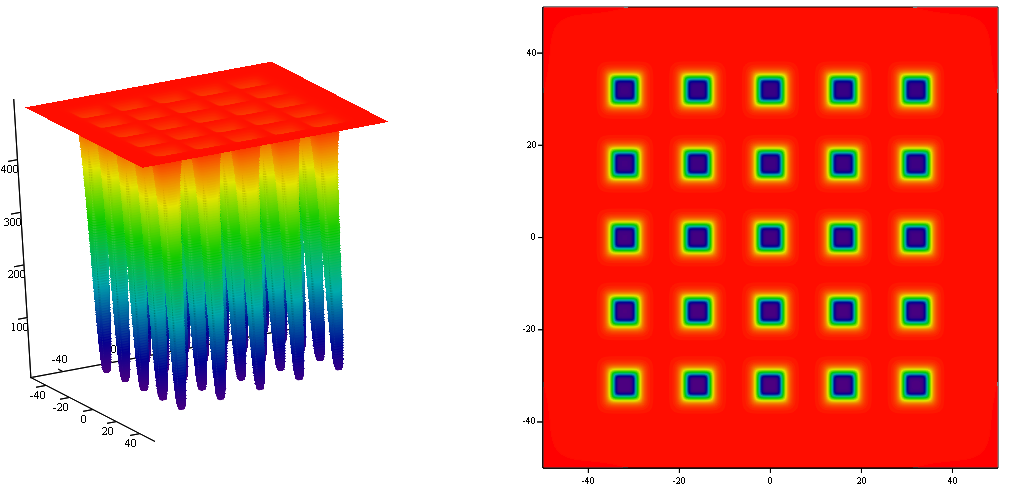
\includegraphics [scale=0.5] {HML_TestFunction_ShekelsFoxholes}
  \caption{Функция <<Лисьи норы>> Шекеля} 
  \label{TestFunctions:img:HML_TestFunction_ShekelsFoxholese}  
\end{figure}

\subsection {Параметры для алгоритмов оптимизации}

\begin{tabularwide}
\textbf{Точность вычислений:} & $\varepsilon=0.25$. \\
\textbf{Число интервалов, на которые предполагается разбивать каждую компоненту вектора $\bar{x}$ в пределах своего изменения} (для алгоритмов дискретной оптимизации) : & $NumberOfParts_j=4095$ ($j=\overline{1,n}$). \\
\textbf{Для этого длина бинарной строки для $x_j$ координаты равна} (для алгоритмов бинарной оптимизации) : & $\left( k_2\right)_j=12$ ($j=\overline{1,n}$). \\
\end{tabularwide}

\textbf{Замечание:}  $NumberOfParts_j$ выбирается как минимальное число, удовлетворяющее соотношению:
\begin{equation*}
NumberOfParts_j=2^{\left( k_2\right)_j }-1\geq\dfrac{10\left( Right_j-Left_j\right) }{\varepsilon},\text{где } \left( k_2\right)_j \in \mathbb{N}, \left( j=\overline{1,n}\right).
\end{equation*}

\subsection {Основная задача и подзадачи}

\begin{tabularwide}
\textbf{Изменяемый параметр: } & $n$ --- размерность вещественного вектора. \\
\textbf{Значение в основной задаче:} & $n=2$.\\
\end{tabularwide}

\subsection {Нахождение ошибки оптимизации}

Пусть в результате работы алгоритма оптимизации за $N$ запусков мы нашли решения $\bar{x}_{submin}^k$ со значениями целевой функции $f\left( \bar{x}_{submin}^k\right) $ соответственно ($k=\overline{1,N}$). Используем три вида ошибок:

\textbf{Надёжность: }
\begin{equation*}
R = \dfrac{\sum_{k=1}^{N}S\left( \bar{x}_{submin}^k \right) }{N}, \text{ где}
\end{equation*}
\begin{equation*}
S\left( \bar{x}_{submin}^k \right)=\left\lbrace \begin{aligned} 1,& \text{ если } \left| \left( \bar{x}_{submin}^k \right)_j-\left( \bar{x}_{min} \right)_j\right|<\varepsilon, j=\overline{1,n};   \\ 0,& \text{ иначе}. \end{aligned}\right.
\end{equation*}

\textbf{Ошибка по входным параметрам:}
\begin{equation*}
E_x = \dfrac{\sum_{k=1}^{N} \left( \frac{\sqrt{\sum_{j=1}^{n}{\left( \left( \bar{x}_{submin}^k \right)_j-\left( \bar{x}_{min} \right)_j \right)}^2 }}{n} \right)  }{N}.
\end{equation*}

\textbf{Ошибка по значениям целевой функции: }
\begin{equation*}
E_f = \dfrac{\sum_{k=1}^{N} \left| f\left( \bar{x}_{submin}^k \right)-f\left( \bar{x}_{min} \right) \right|  }{N}.
\end{equation*}

\subsection {Свойства задачи}
\begin{tabularwide}
\textbf{Условной или безусловной оптимизации: } & Задача безусловной оптимизации. \\
\textbf{Одномерной или многомерной оптимизации: } & Многомерной: (двумерной). \\
\textbf{Функция унимодальная или многоэкстремальная: } & Функция многоэкстремальная. \\
\textbf{Функция стохастическая или нет: } & Функция не стохастическая. \\
\textbf{Особенности: } & Глобальный минимум слабо отличается от локальных. Из локальных минимумов алгоритмам обычно сложно выбраться.\\
\end{tabularwide}

\subsection {Реализация}

Реализация функции взята из библиотеки HarrixMathLibrary в разделе <<Тестовые функции для оптимизации>>, которую можно найти по адресу \href{https://github.com/Harrix/HarrixMathLibrary} {https://github.com/Harrix/HarrixMathLibrary}.

\begin{lstlisting}[caption=Код функции HML\_TestFunction\_ShekelsFoxholes]
double HML_TestFunction_ShekelsFoxholes(double x, double y)
{
/*
Функция двух переменных: функция "Лисьи норы" Шекеля.
Тестовая функция вещественной оптимизации.
Входные параметры:
 x - первая вещественная переменная;
 y - вторая вещественная переменная.
Возвращаемое значение:
 Значение тестовой функции в точке (x,y).
*/
double VHML_Result;
double K=500.;
double f1,f2;
int j,k;
int a[2][25];

a[0][0]=-32;
a[0][1]=-16;
a[0][2]=0;
a[0][3]=16;
a[0][4]=32;
a[0][5]=-32;
a[0][6]=-16;
a[0][7]=0;
a[0][8]=16;
a[0][9]=32;
a[0][10]=-32;
a[0][11]=-16;
a[0][12]=0;
a[0][13]=16;
a[0][14]=32;
a[0][15]=-32;
a[0][16]=-16;
a[0][17]=0;
a[0][18]=16;
a[0][19]=32;
a[0][20]=-32;
a[0][21]=-16;
a[0][22]=0;
a[0][23]=16;
a[0][24]=32;

a[1][0]=-32;
a[1][1]=-32;
a[1][2]=-32;
a[1][3]=-32;
a[1][4]=-32;
a[1][5]=-16;
a[1][6]=-16;
a[1][7]=-16;
a[1][8]=-16;
a[1][9]=-16;
a[1][10]=0;
a[1][11]=0;
a[1][12]=0;
a[1][13]=0;
a[1][14]=0;
a[1][15]=16;
a[1][16]=16;
a[1][17]=16;
a[1][18]=16;
a[1][19]=16;
a[1][20]=32;
a[1][21]=32;
a[1][22]=32;
a[1][23]=32;
a[1][24]=32;

VHML_Result=1./K;
for (j=0;j<25;j++)
 {
 f1=1;
 for (k=0;k<6;k++) f1=f1*(x-a[0][j]);
 f2=1;
 for (k=0;k<6;k++) f2=f2*(y-a[1][j]);
 VHML_Result+=1./(j+1.+f1+f2);
 }
 
VHML_Result=1./VHML_Result;

return VHML_Result;
}
\end{lstlisting}

\subsection {Ссылки}

Данная функция приводится в следующих источниках:

\begin{enumerate}
\item \cite[стр. 34]{book:Semenkin2007} ---  \href{http://files.lib.sfu-kras.ru/ebibl/umkd/22/u_lectures.pdf}{Эволюционные методы моделирования и оптимизации сложных систем}.
\item \cite[стр. 729]{book:huang2006international} ---  \href{http://books.google.ru/books?id=7sH4RsXYu7cC}{International Conference on Intelligent Computing: Intelligent computing}.
\end{enumerate}